% !TeX document-id = {a90a2b0a-e08e-44ed-850a-35793bedbf3a}
% !TeX TS-program = xelatex

% !BIB program = biber
\documentclass[handout]{beamer}
%\documentclass[compress]{beamer}
\usepackage[T1]{fontenc}
\usepackage{pifont}
\usetheme[block=fill,subsectionpage=progressbar,sectionpage=progressbar]{metropolis} 


\definecolor{Purple}{HTML}{911146}
\definecolor{Orange}{HTML}{CF4A30}

% Theme colors are derived from these two elements
\setbeamercolor{alerted text}{fg=Orange}

% ... however you can of course override styles of all elements
\setbeamercolor{frametitle}{bg=Purple}


\usepackage{wasysym}
\usepackage{etoolbox}
\usepackage[utf8]{inputenc}

\usepackage{threeparttable}
\usepackage{subcaption}

\usepackage{tikz-qtree}
\setbeamercovered{still covered={\opaqueness<1->{5}},again covered={\opaqueness<1->{100}}}


\usepackage{listings}

\lstset{
	basicstyle=\scriptsize\ttfamily,
	columns=flexible,
	breaklines=true,
	numbers=left,
	%stepsize=1,
	numberstyle=\tiny,
	backgroundcolor=\color[rgb]{0.85,0.90,1}
}



\lstnewenvironment{lstlistingoutput}{\lstset{basicstyle=\footnotesize\ttfamily,
		columns=flexible,
		breaklines=true,
		numbers=left,
		%stepsize=1,
		numberstyle=\tiny,
		backgroundcolor=\color[rgb]{.7,.7,.7}}}{}


\lstnewenvironment{lstlistingoutputtiny}{\lstset{basicstyle=\tiny\ttfamily,
		columns=flexible,
		breaklines=true,
		numbers=left,
		%stepsize=1,
		numberstyle=\tiny,
		backgroundcolor=\color[rgb]{.7,.7,.7}}}{}


\usepackage[american]{babel}
\usepackage{csquotes}
\usepackage[style=apa, backend = biber]{biblatex}
\DeclareLanguageMapping{american}{american-UoN}
\addbibresource{../literature.bib}
\renewcommand*{\bibfont}{\tiny}

\usepackage{tikz}
\usetikzlibrary{shapes,arrows,matrix}
\usepackage{multicol}

\usepackage{subcaption}

\usepackage{booktabs}
\usepackage{graphicx}

\graphicspath{{../pictures/}}

\makeatletter
\setbeamertemplate{headline}{%
	\begin{beamercolorbox}[colsep=1.5pt]{upper separation line head}
	\end{beamercolorbox}
	\begin{beamercolorbox}{section in head/foot}
		\vskip2pt\insertnavigation{\paperwidth}\vskip2pt
	\end{beamercolorbox}%
	\begin{beamercolorbox}[colsep=1.5pt]{lower separation line head}
	\end{beamercolorbox}
}
\makeatother



\setbeamercolor{section in head/foot}{fg=normal text.bg, bg=structure.fg}



\newcommand{\question}[1]{
	\begin{frame}[plain]
		\begin{columns}
			\column{.3\textwidth}
			\makebox[\columnwidth]{
				
\includegraphics[width=\columnwidth,height=\paperheight,keepaspectratio]{../pictures/mannetje.png}}
			\column{.7\textwidth}
			\large
			\textcolor{orange}{\textbf{\emph{#1}}}
		\end{columns}
\end{frame}}

\newcommand{\instruction}[1]{\emph{\textcolor{gray}{[#1]}}}


\title[Computational Communication Science 2]{\textbf{Computational Communication Science 2} \\Week 8 - Lecture\\ »A Deep Dive into Supervised Machine Learning«}
\author[Marthe Möller, Anne Kroon]{Marthe Möller \\ Anne Kroon \\ ~ \\ \footnotesize{a.m.moller@uva.nl, @marthemoller \\a.c.kroon@uva.nl, @annekroon} \\}
\date{May, 2022}
\institute[Digital Society Minor, University of Amsterdam]{Digital Society Minor, University of Amsterdam}


\begin{document}
	
	\begin{frame}{}
		\titlepage
\end{frame}
	
\begin{frame}{Today}
		\tableofcontents
\end{frame}


\section{Recap}

\begin{frame}{Recap}
	
Last week, we talked about:
	\begin{itemize}
		\item Supervised Machine Leaning (SML)
		\item The principles behind SML
		\item The steps of SML
		\item Some commonly used ML models
		\item Validating models \\\
	\end{itemize}
	
At home, you:
	\begin{itemize}
		\item Got some hands-on experience SML (homework assignment)
	\end{itemize}
	
\end{frame}


\begin{frame}{Recap}
	
Today, we:
	\begin{itemize}
		\item Your first SML experience
		\item Take a deep dive into validating SML-models
		\item Take a critical look at SML 
	\end{itemize}
	
\end{frame}


\begin{frame}{Recap}
	
This week, you practiced with code that:
\begin{itemize}
	\item Imported all required packages and modules needed to run the script (Q1)
	\item Read in some data (Q2)
	\item Set up a Count vectorizer (Q3)
	\item Trained a Naïve Bayes model with the count vectorizer and requested some metrics for validation (Q4)
	\item Set up a tf-idf vectorizer, used it in a LogRegression model and requested some metrics for validation (Q5)
\end{itemize}
	
\end{frame}


\begin{frame}[fragile]{Recap Q1}
	
\begin{lstlisting}
import csv
from collections import Counter
import matplotlib.pyplot as plt
from sklearn.feature_extraction.text import (CountVectorizer, TfidfVectorizer)
from sklearn.naive_bayes import MultinomialNB
from sklearn.metrics import accuracy_score
from sklearn.linear_model import (LogisticRegression)
from sklearn.metrics import confusion_matrix,classification_report
from sklearn.pipeline import (make_pipeline, Pipeline)
from sklearn.model_selection import GridSearchCV
import pickle
import joblib
\end{lstlisting}
	
Why import all modules at the start of a Python Script?
\end{frame}


\begin{frame}[fragile]{Recap Q2}
Read in the ingredients for SML (dataset is already split):
\begin{lstlisting}
test = "test.txt"
train = "train.txt"

texts_test = []
labels_test = []

with open(test) as fi:
     data = csv.reader(fi, delimiter=';')
     for row in data:
          texts_test.append(row[0])
          labels_test.append(row[1])

\end{lstlisting}

Mind: Choose the correct delimiter (e.g., ';', ',', '\textbackslash t'). \\
IndexError: list index out of range' often pops up if you choose the wrong one.
\end{frame}


\begin{frame}[fragile]{Recap Q2}
What happens here?
\begin{lstlisting}
len(texts_test) == len(labels_test)
len(texts_train) == len(labels_train)
\end{lstlisting}
	
\begin{lstlistingoutput}
TRUE
\end{lstlistingoutput}.
\end{frame}


\begin{frame}[fragile]{Recap Q2}
Why would you do this?
\begin{lstlisting}
plt.bar(Counter(labels_train).keys(), Counter(labels_train).values())
\end{lstlisting}
	
\end{frame}



\begin{frame}[fragile]{Recap Q3}
Remember, the computer can't read words! We need to transform the texts and labels into vectorizers.
\begin{lstlisting}
countvectorizer = CountVectorizer(stop_words="english")
X_train = countvectorizer.fit_transform(texts_train)
X_test = countvectorizer.transform(texts_test)
\end{lstlisting}

When fit\_transform and when transform?
\end{frame}


\begin{frame}[fragile]{Recap Q4}
The actual SML part (yes, truly, it is three lines of code!):
\begin{lstlisting}
nb = MultinomialNB()
nb.fit(X_train, labels_train)
y_pred = nb.predict(X_test)
\end{lstlisting}
	
No output?
\end{frame}

\begin{frame}[fragile]{Recap Q4}
You can check what was created:
\begin{lstlisting}
print(y_pred[:10])
\end{lstlisting}

\begin{lstlistingoutput}
['sadness' 'sadness' 'sadness' 'joy' 'sadness' 'fear' 'sadness' 'joy' 'joy' 'sadness']
\end{lstlistingoutput}
\end{frame}


\begin{frame}[fragile]{Recap Q4}

\begin{lstlisting}
accuracy = accuracy_score(labels_test, y_pred)
print(accuracy)
\end{lstlisting}
	
\begin{lstlistingoutput}
0.7945
\end{lstlistingoutput}
\end{frame}


\begin{frame}[fragile]{Recap Q5}
Repeat with a different vectorizer and a different SML model!
\begin{lstlisting}
tfidfvectorizer = TfidfVectorizer(stop_words="english")
X_train = tfidfvectorizer.fit_transform(texts_train)
X_test = tfidfvectorizer.transform(texts_test)

logres = LogisticRegression()
logres.fit(X_train, labels_train)
y_pred = logres.predict(X_test)

print(classification_report(labels_test, y_pred))
\end{lstlisting}
	
\end{frame}


\begin{frame}{Up next}
In the remainder of the exercise, you will:
\begin{itemize}
\item Write down code to compare different vectorizers/models in an effective way (Q6)
		\item Learn about hyperparameters in vectorizers (Q7)
		\item Practice with cross-validation and gridsearch (Q8 \& Q9)
		\item Saving vectorizers and classifiers (Q10) 
\end{itemize}

Cross-validation? Hyperparameters? Gridsearch?
\end{frame}


%\section{SML in practice}

%\begin{frame}{Neural Networks}
	
%	\begin{center}
%		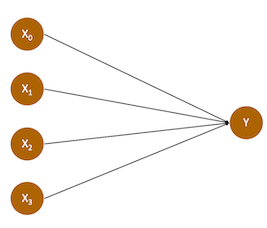
\includegraphics{../pictures/perceptron.png} \\\
%	\end{center}
	
	% What does a computer actually do with the models discussed above? In this lecture, we discuss neural networks as a machine learning algorithm.
	
	% Neural networks consist of connection between neurons that are activated if the total input is above a certain threshold. Simplest form: perceptron.
	
	% A perceptron is a single-layer neural network.
	
	% Input neurons (or IV’s) connected to an output neuron (or DV). Each of the connections between neurons has a weight which can be positive or negative. For the output neuron, the weighted sum of inputs is calculated and a function is applied to determine the results. Which function is not set, it could be, for example, a logistic regression!
	
%\end{frame}


%\begin{frame}{Neural Networks}
	
%	\begin{center}
%		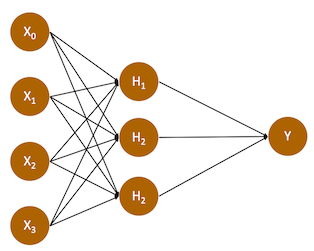
\includegraphics{../pictures/neuralnetwork_hiddenlayer.png} \\\
%	\end{center}
	
%	\begin{tiny}
%		\fullcite{ha_automatically_2021} 
%	\end{tiny}
	
	% Imagine we use machine learning to determine the positivity or negativity of online movie reviews (sentiment analysis). The input neurons could be the frequencies of words such as “great” (positive weight) and “horrible” (negative weight). Such a network is a bit simplistic, because a review that says something is “not great” is negative but this wouldn’t be picked up by our network.
	
	% To solve this, we can add a hidden layer of latent variables between the input and the output layer of the network.
	
	% Connect to Ha et al. (link to deep learning)
	
	
%\end{frame}


\section{More about validation}

\begin{frame}{Finding the best performing model}

We talked about validating models based on various metrics, such as accuracy, F1-score, precision, recall... \\\

What is the most important metric when deciding what model is best?
\end{frame}



\begin{frame}{Finding the best performing model}

\begin{center}
	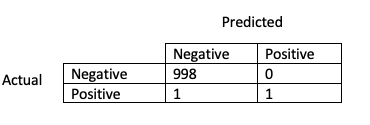
\includegraphics[width=\linewidth,height=\textheight,keepaspectratio]{../pictures/ConfusionMatrix1.png} \\\
\end{center}

Accuracy: In which percentage of all cases was our classifier right? 

%Very high accuracy, yay!
% But what if the true positive was some with a very contagious virus that can spread super quickly?

\end{frame}



\begin{frame}{Finding the best performing model}
\begin{center}
	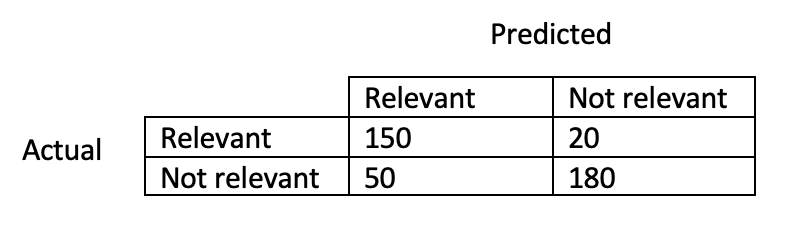
\includegraphics[width=\linewidth,height=\textheight,keepaspectratio]{../pictures/ConfusionMatrix2.png} \\\
\end{center}
	
Recall: How many of the cases that we wanted to find did we actually find? \\\
Here: 0.88
	
% Pretty high recall, but we missed quite a bit of relevant documents here - this may cause problems in my study? 
	
\end{frame}



\begin{frame}{Finding the best performing model}
	\begin{center}
		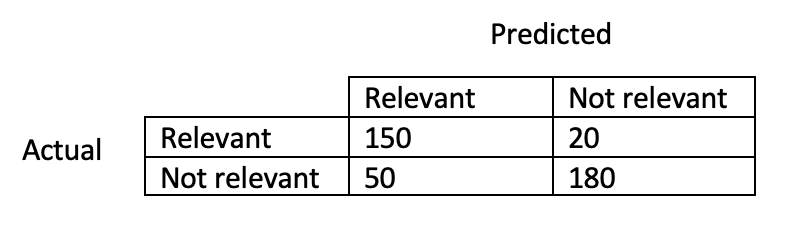
\includegraphics[width=\linewidth,height=\textheight,keepaspectratio]{../pictures/ConfusionMatrix2.png} \\\
	\end{center}
	
	Precision:  How much of what we found is actually correct? \\\
	Here: 0.75
	
	% Pretty high recall, but 25% of our labels are incorrect - this may cause problems in my study? 
	
\end{frame}


\begin{frame}{Finding the best performing model}

What if it is hard to say which one is most important and you want to find a balance between precision and recall?

F1- score!
		
\end{frame}



\section{Cross-validation}

\begin{frame}{Cross-validation}
	
	Overfitting: When a model fits \emph{exactly} against the data.
	
	When we calculate the metrics discussed above for multiple models on the same test dataset, we run the risk of overfitting on the test data.
	
	%Consequence of this is, for example, that your model can classify your training data perfectly, but it can't classify other data very well anymore.
	
	%Overfitting the model generally takes the form of making an overly complex model to explain idiosyncrasies in the data under study. In reality, the data often studied has some degree of error or random noise within it. Thus, attempting to make the model conform too closely to slightly inaccurate data can infect the model with substantial errors and reduce its predictive power.
	
\end{frame}


\begin{frame}{Cross-validation}
	
	Potential solution: Split the dataset into three smaller sets. A training dataset, a validation dataset and a test dataset.
	
	However, this requires us to have a very large labeled dataset. In reality, this is not always the case!
	
\end{frame}


\begin{frame}{Cross-validation}
	
	Cross-validation: A resampling procedure to evaluate ML models on a limited data sample.
	
	\(k\)-fold cross-validation, where \(k\) refers to the number of groups or folds in which a sample is split.

\end{frame}


\begin{frame}{\(k\)-fold cross-validation}
	\(k\)-fold cross-validation step by step:
	\begin{enumerate}
		\item Shuffle the data
		\item Split the data into \(k\) folds (groups)
		\item For each unique group
		\begin{enumerate}
			\item Take the group as a test dataset
			\item Take the remaining groups as one training dataset
			\item Fit a model on the training set and evaluate it on the test set
			\item Retain the evaluation score and discard the model
		\end{enumerate}
		\item Summarize the evaluation scores to assess the model \\\
	\end{enumerate}

\end{frame}
	

\begin{frame}{Cross-validation}
	
	Cross-validation is often used to compare many different model specifications, for example to find the best hyperparameters.
	
	Hyperparameters: Parameters of the model that are not estimated from the data. 
	
	To do this, the Grid Search algorithm is often used.
	
\end{frame}


\begin{frame}{Grid Search}
	
The GridSearchCV module (scikit-learn) searches for the best values of specified parameters using cross-validation.

The outcome is the optimal combination of one or more parameters.
	
\end{frame}



\begin{frame}{Zooming out} 
	
	We talked about:
	\begin{itemize}
		\item Your experience with SML so far
		\item Cross-validation and grid search \\\
	\end{itemize}
	
	Next, we will talk about:
	\begin{itemize}
		\item Strengths and challenges associated to SML
	\end{itemize}
	
\end{frame}


\section{SML: Strenghts and Challenges}


\begin{frame}{Strengths and Challenges} 
	
Strengths?

	
Challenges?

\end{frame}



\begin{frame}{Strengths and Challenges} 
	
Strengths:
\begin{itemize}
	\item Easier to code large datasets
	\item Enhances replicable research
	\item Easier to study "natural" human behavior \\\
\end{itemize}
	
Challenges:
\begin{itemize}
	\item Resource constraints
	\item Ethical considerations
	\item Criticism required (see next slide)
\end{itemize}

% Strengths:
% -	Makes it easier to code large datasets (cheaper, faster)
% -	Enhances replicable research (exactly the same script can be used to by researchers to conduct a new content analysis)
% -	Makes it easier to study “natural” human behavior (example: study social influence by hiring actors to see if it influences people’s reactions to videos; now, we can just analyze the comments people write and how these influence subsequent comments!)

% Challenges
% -	(Jordan & Mitchell, p. 5) Resource constraint (privacy, required processing capacities  communication constraint
% -	Ethical questions: Who will have access to, and ownership of, online data and who will reap its benefits? (Jordan & Mitchell, p.6)

\end{frame}


\begin{frame}{Strengths and Challenges}
	
	
\begin{center}
	\includegraphics[width=\linewidth,height=\textheight,keepaspectratio]{../pictures/ericsson.png} \\\
\end{center}

\end{frame}
	


\begin{frame}{Strengths and Challenges}
	\begin{center}
		
\includegraphics[width=\linewidth,height=\textheight,keepaspectratio]{../pictures/toeslagenaffaire_headlines.png} \\\
	\end{center}
	
% As shown by Jordan & Mitchell, ML is used in many different facets of society. But it is impertinent that those who use ML remain critical of its capabilities. If a machine is trained based on human coded data, as is the case with SML, it will also learn about the prejudices that humans have: toeslagenaffaire voorbeeld. Laag inkomen werd door computer geleerd als voorspeller van fraude. Mensen met een laag inkomen werden er dus bij voorbaat al uitgepikt. 
%  Remember that in the end, machines are created by humans and as humans we are responsible for how we use them. We have the responsibility to ask questions about what machines do and how and whether we should!
	
\end{frame}


\section{Looking back and ahead}

\begin{frame}{Zooming out} 
	
	We talked about:
	\begin{itemize}
		\item The principles behind SML
		\item Some frequently used SML models
		\item Validating SML classifiers
		\item SML in practice
		\item Cross-validation and grid search
		\item Strengths and challenges associated to SML \\\
\end{itemize}
	

\end{frame}


\begin{frame}{Zooming out} 
	
This week's tutorial:
	\begin{itemize}
		\item Hands-on approach to take a further look into the machine learning process
		\item Questions about prior tutorial exercises
	\end{itemize}
	
\end{frame}


\begin{frame}{Looking back} 
	
You started with the basics (e.g., what is a list, how to save data, write a loop).\\
In two months, you learned:
	\begin{itemize}
		\item How to read in data
		\item How to preprocess data
		\item How transform text into data that a computer can understand
		\item How to compare texts to provide a recommendation
		\item How to analyze text to classify it automatically
	
	\end{itemize}
	
\end{frame}


\begin{frame}{Looking at the very near future} 
	
One last grade for this course, the take-home exam.
	\begin{itemize}
		\item The take-home exam will be published on 30 May (9 am)
		\item The deadline for submitting the take-home exam is on 2 June (9 am)
		\item The exam covers materials discussed in weeks 1 through 7 (but you may of course also use anything you learned in week 8, this is not required, however) 
	\end{itemize}
	
\end{frame}

\begin{frame}{Looking at the near future} 
	
Final course of the minor: the research project!
\begin{itemize}
		\item You will combine your programming skills with your skills as a researcher
		\item Run a research project about ComScience using the materials you created for the group assignment in this course
		\item More information follows in the first meeting of the research project
\end{itemize}
\end{frame}

\begin{frame}{Looking at the future} 
	
CCS-1 and CCS-2: An introduction to coding. You can continue to learn and work with Python.\\
No course materials and instructors to help you out, but there are a lot of resources online!\\
Our tips:
	\begin{itemize}
		\item Error message? Google is your best friend!
		\item Check out the documentation of any module that you use to learn how it works
		\item Check out pubs using the method you are interested in. Often, they publish their python scripts (e.g., Meppelink et al., 2021)
	\end{itemize}
	
\end{frame}



\begin{frame}{Looking at the future} 
	
Thank you for the past weeks and enjoy the research project!

\end{frame}





\end{document}